% Copyright (c) 2008-2009 solvethis
% Copyright (c) 2010-2011 Casper Ti. Vector
% Public domain.

\chapter{背景介绍与相关工作}
本章将介绍WiFi的背景、WiFi安全的研究进展以及相关的WiFi验证平台。
本章首先在\ref{sec:comm_principle}节、\ref{sec:80211protocol}节介绍WiFi的背景知识,
然后在\ref{sec:security_research}节介绍物理层WiFi安全相关的研究,
其次在\ref{sec:related_work}节介绍现有的WiFi验证平台,
最后在\ref{sec:chap2_conclusion}节对本章进行小结。

	\section{WiFi物理层信息}\label{sec:comm_principle}
	研究者利用物理层信息加强WiFi的安全性,不同的物理层信息各有特点。
	本节介绍在WiFi安全研究中常见的几种物理层信息及其在无线通信中的物理意义。
		\subsection{RSS与RSSI}
		RSS(Received Signal Strength)是接收信号强度,指WiFi接收机收到的信号的功率,
		单位为dBm,为负数,越接近0表示信号质量越高。
		RSSI(Received Signal Strength Indicator)是接收信号强度指示,是无单位的。
		RSS一般为负值不太直观,人们把RSS人为映射为正值RSSI,理解和比较起来更直观,
		一般WiFi系统呈现给用户的是RSSI,不同系统有不同的映射方式\cite{wikirssi}。
		RSSI本质上与RSS只是同一个物理层信息的不同表示方法,文献里用二者都会出现,本文以RSSI进行表示。

		RSSI与无线发射机功率、收发距离、周围障碍物环境有关,发射机功率越大、收发距离越短,RSSI越大,而RSSI与障碍物环境关系比较复杂。
		不同的位置来源的信号一般RSSI也不同,因此无线通信的研究者常常通过RSSI获取相对位置。

		\subsection{CSI与CIR}\label{sec:background_csi}
		CSI(Channel State Information)是信道状态信息,是无线通信中从发射机到接收机之间信道的属性。
		在无线通信中,接收机接收到的信号与发送信号不完全相同,存在环境引起的变化,
		环境的影响称为信道,接收信号是发送信号与信道共同作用的结果,如式\ref{math:channel_model},
		\begin{equation}
			\centering
			r(t)=h(t)*s(t)+n
			\label{math:channel_model}
		\end{equation}
		$r(t)$代表接收信号,$h(t)$代表信道,$s(t)$代表发送信号,$n$代表噪声。

		接收机为了从接收信号中还原出发送信号,需要先得到信道信息,然后消除信道对接收信号的影响。
		接收机得到的信道信息,称作CSI。
		为了得到CSI,无线通信中常采用的方法是发射机发送一段双方已知的信号,称为训练序列,接收机对比接收信号和理论信号,
		得到信道信息,这个过程称为信道估计,从接收信号中消除信道影响的过程称为补偿\cite{book06commprin}。
		这里基于的一个假设是在短时间内信道变化不大,信道对训练序列的作用与信道对信号其它部分的作用相近。

		影响CSI的因素很多,有多径效应、多普勒效应、随距离的能量衰减等。
		多径效应是指由于周围物体的反射,信号经过多条路径到达接收机,每条路径效果叠加称为多径效应\cite{book06commprin}。
		多普勒效应是由发射机和接收机之间相对位置的变化引起。
		CSI具有丰富的物理内涵,常常被无线研究者用来推测其它信息,比如判断位置、判断是否有人经过、判断是否在移动。

		有的文献中也具体标明使用CIR这个物理量,CIR(Channel Impulse Response)是信道冲激响应,是一种特殊的CSI
		表示发送端发送一个脉冲信号的时候,接收端所能收到的信号值$h(t)$。
		CIR通常表示时域的信道特征,CSI既包含时域特征,也包含频域特征,是信道信息的总称。

		\subsection{频率偏移}
		介绍频率偏移之前,首先介绍频率同步。同步是指无线通信系统的接收机从收到的波形中找出有效信号,是无线通信中必不可少的步骤。
		同步分为两类,时间同步和频率同步。时间同步是指找到发送信号的起始时间,对于异步的通信系统都需要进行时间同步,如串口通信协议。
		接收信号和发送信号的载波频率存在频率偏移(简称频偏),频率同步是指找到并补偿频率偏移,还原出发送信号。
		频偏对频分复用系统会造成很严重的影响,因此频率同步是频分复用系统必要的组成部分。

		\begin{figure}[H]
			\centering
			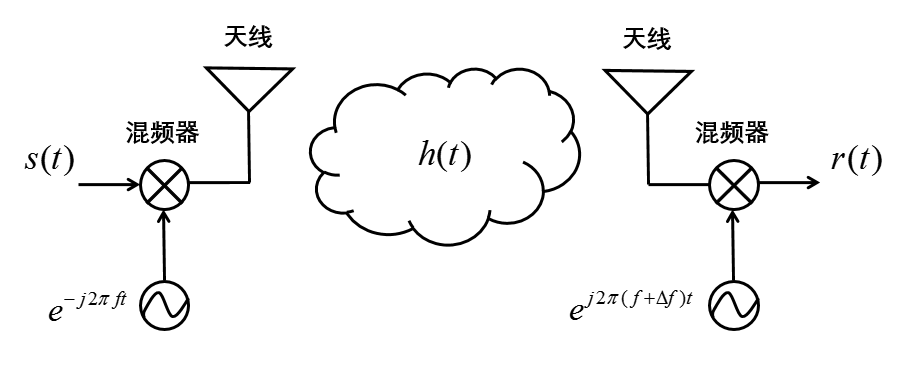
\includegraphics[width=0.7\textwidth]{img/freq_offseet_channel_model.png}
			\caption{无线通信系统中频率偏移的信道模型}
			\label{fig:freq_offseet_channel_model}
		\end{figure}
		频偏的信道模型可以由图\ref{fig:freq_offseet_channel_model}表示,$s(t)$表示发送的基带信号,$r(t)$表示接收的基带信号,$h(t)$表示信道,
		混频器用来将基带信号与载波合成后搬移到射频上,图中省略了低噪声放大器等其他通信电路。
		如图\ref{fig:freq_offseet_channel_model}所示,频率偏移由接收机和发射机载波频率不一致引起,
		设发射机载波频率为$f$,接收机载波频率为$f+\Delta f$,$\Delta f$为频率偏移。
		频偏的数学模型可以表示为式\ref{math:freq_offset},噪声对频偏几乎没有影响,
		\begin{equation}
			\centering
			r(t)=h(t)*s(t) \cdot e^{-j2\pi ft} \cdot e^{j2\pi(f+\Delta f)t}
			\label{math:freq_offset}
		\end{equation}
		对于实际的无线通信系统,常常使用有周期性的训练序列进行频偏估计,根据周期的偏移推测频率偏移,然后进行频偏补偿。

	\section{802.11协议简介}\label{sec:80211protocol}
	WiFi通信的协议是IEEE 802.11协议集,规定了MAC(媒体访问控制)层和物理层的规范,
	具体协议按推出的时间顺序有802.11b、802.11a、802.11g、802.11n、802.11ac等。
	目前市面上的主流WiFi芯片都支持802.11a/g/n协议,本文主要基于802.11a/g/n协议进行阐述。
		\subsection{802.11物理层介绍}
		802.11物理层规定了数据传输的调制解调方式、编码方式、射频参数等,是OSI网络模型的最底层。
		除802.11b使用DSSS(direct-sequence spread spectrum,直接序列扩频)调制技术外,
		802.11a/g/n/ac等都使用了OFDM(Orthogonal frequency-division multiplexing,正交频分复用)调制技术。

		OFDM是一种将信号分配到多个子载波的频分调制方式,每一个子载波的调制后信号有部分重叠,但因为子载波之间严格正交,接收机可以分离出不同子载波的信号。
		OFDM的优点是在子载波间不需要保护间隔,频谱利用率高,且抗多径衰落能力强,
		缺点是对频率偏移敏感,需要对频偏进行纠正\cite{book06commprin}。
		OFDM由于其对复杂环境的抗干扰性,目前广泛应用于宽带通信,如WiFi、4G移动网络、数字电视、非对称数字用户环路(ADSL)等。
		802.11a/g协议规定的OFDM子载波数量为64个,其中传输数据的子载波是48个,传输导频的子载波是4个,
		802.11n协议20M带宽模式下子载波数量为64个,其中传输数据的子载波是52个,传输导频的子载波是4个,
		802.11n协议高吞吐率40M带宽模式下子载波数量为128个,其中传输数据的子载波是108个,传输导频的子载波是6个\cite{ieee80211}。

		\begin{figure}[H]
			\centering
			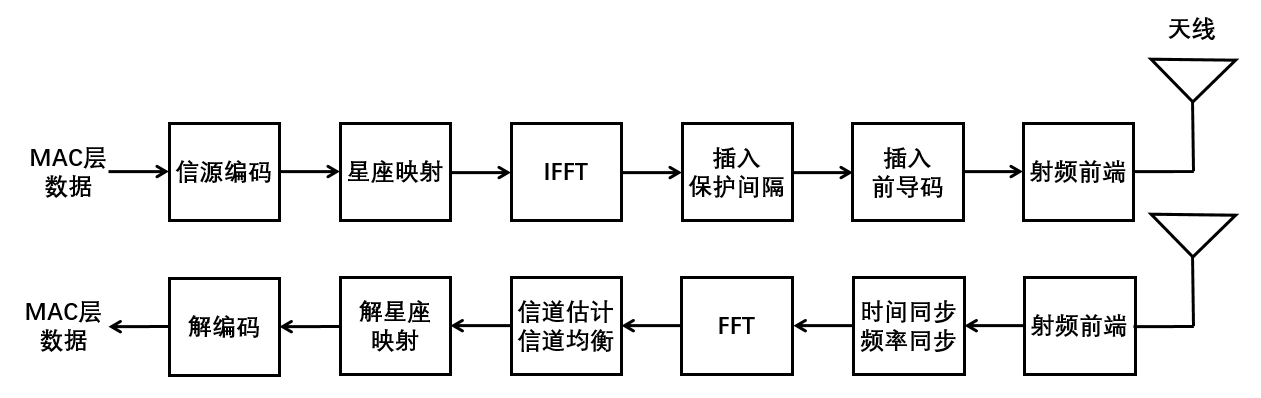
\includegraphics[width=0.7\textwidth]{img/80211_phy_module.png}
			\caption{802.11a/g物理层的简单模块示意图}
			\label{fig:80211_phy_module}
		\end{figure}
		图\ref{fig:80211_phy_module}是802.11a/g物理层的简单模块示意图,802.11n在此基础上增加对多天线的支持。
		发送端得到来自MAC层的数据,经过信源编码、星座映射、IFFT(Inverse Fast Fourier Transform,快速傅里叶逆变换)、插入保护间隔、插入前导码、射频前端到达空气中。
		其中,信源编码包括扰码、冗余编码、交织等步骤,目的是使信源数据更加强健;
		星座映射是将二进制数据映射到复数星座点上,有不同的映射策略,对应多种调制方式;
		IFFT是OFDM的关键步骤,将频域信号转变为时域信号,对于802.11a/g,此处是64点IFFT,对于802.11n,此处兼有64点IFFT和128点IFFT;
		插入保护间隔是指在时域的不同符号间插入一段间隔时间,降低码间串扰的影响;
		插入前导码是指在一帧前面增加训练字,如\ref{sec:comm_principle}节所述,训练字用来完成时间同步、频率同步、信道估计等功能。
		接收端从空气中得到无线信号,经过射频前端得到复数表示的I/Q两路信号,经过时间同步和频率同步后得到一帧,
		去掉保护间隔后经过FFT得到频域信号,经过信道估计和信道均衡后去除信道对信号的影响,
		经过解星座映射后由复数信号得到二进制数据,经过解码还原出真实数据,传给MAC层。

		802.11物理层中蕴含了很多对于WiFi安全研究有价值的信息,尤其是接收端模块,比如信道估计模块可以得到CSI,反映了发射机的位置、周边环境等,
		频率同步模块可以得到频率偏移,解星座映射模块可以得到接收信号的星座图。

		\subsection{802.11 MAC层介绍}
		在OSI网络模型中,物理层之上的一层是数据链路层,MAC层是数据链路层的子层,802.11协议规定的是物理层和MAC层的规范。
		MAC层提供了在不可靠的无线媒介中可靠传输用户数据的机制。本文主要面向物理层,会简单涉及MAC层,此处只对MAC层做简单介绍。

		802.11 MAC层有两种功能规范,必须具备的功能DCF(Distributed Coordination Function,分布式协调功能)
		和可选功能PCF(Point Coordination Function,集中式协调功能)。
		DCF主要基于CSMA/CA(Carrier sense multiple access with collision avoidance,带碰撞避免的载波侦听多址)技术。
		CSMA/CA技术是指一个无线节点在发送数据之前,首先侦听当前载波上是否有其他设备使用,只有没有其他人发送时可以发送数据。
		当有其他人发送数据时,首先等到空闲,然后再等待随机一段时间空闲后再发送,随机等待机制称为随机回退\cite{citsa05backoff}。

		\subsection{802.11安全机制}\label{subsec:80211security}
		802.11协议在MAC层规定了安全机制。
		1997年推出的最初的802.11协议将WEP(Wired Equivalent Privacy)认证方式应用于MAC层规范,
		后来在2003年,WiFi联盟提出WPA(Wi-Fi Protected Access)认证方式,
		在2004年,随着IEEE推出802.11i协议规定了WPA2认证方式,WEP认证被弃用\cite{wikiwep},
		在2012版802.11协议中,只保留WPA2认证方式,即802.11i协议\cite{ieee80211}。

		WEP和WPA被802.11协议弃用是因为其强度低易被破解,然而,WPA2认证方式也存在被攻击的可能。
		\cite{ijarcet12wpa2}中研究了WEP、WPA、WPA2的漏洞,并利用软件Aircrack-ng演示了如何破解这三种认证方式。
		MAC层安全机制的不完备性驱动越来越多的研究者开始探索物理层的安全机制,在第\ref{sec:security_research}节会介绍相关研究。

	\section{物理层WiFi安全研究进展}\label{sec:security_research}
	本节首先在\ref{subsec:attack_model}小节介绍WiFi攻击模型的研究进展,提出新的攻击模型是巩固WiFi安全的一种方式;
	其次介绍物理层WiFi安全机制的研究进展,研究者利用物理层信息进行用户的认证和设备的识别,
	物理层安全机制分为基于加密技术的安全机制和非加密安全机制,基于加密技术的安全机制在\ref{subsec:phy_tech_key_generation}小节进行介绍,
	非加密安全机制可以宽泛地分为硬件指纹技术和信道指纹技术\cite{ieeewc10noncryp}\cite{mobicom08radiometric},分别在
	\ref{subsec:phy_tech_device_fingerprint}、\ref{subsec:phy_tech_channel_fingerprint}小节进行介绍。
		\subsection{WiFi攻击模型的研究进展}\label{subsec:attack_model}
		相对于有线网络,无线网络的开放性给攻击者带来了可乘之机。针对WiFi的攻击按主动性可分为被动攻击和主动攻击。
		被动攻击主要是窃听获取密码,
		例如,通过监听CSI和上层网络报文,可以推测出用户在手机支付时输入的密码\cite{ccs16csi};
		通过窃听相邻设备的信道信息,获取基于信道的加密密钥\cite{ccs07robustkey}。
		主动攻击有欺骗攻击、DoS(Denial of Service,拒绝服务)攻击、密钥破解等,
		例如:攻击者伪装成合法设备MAC地址,只用10秒钟向AP发送去认证包,可使合法设备数分钟内无法连接AP\cite{usenix03dos};
		攻击者产生大量随机MAC地址向AP发送连接请求,消耗网络资源,可使DHCP服务器可分配IP被全部消耗\cite{wisec06spoofing};
		攻击者发起DoS攻击,不停地发送干扰信号,使合法设备之间无法正常通信\cite{milcom13jamming, jsac12antijamming};
		信号注入攻击可以破解密钥,攻击者通过向密钥达成一致的两台设备之间注入无线信号,
		使合法设备生成被自己控制的密钥,攻击者很大概率可以猜出密钥\cite{cns15key}。

		\subsection{物理层密钥技术}\label{subsec:phy_tech_key_generation}
		物理层密钥技术是指利用物理层信息生成密钥,对通信内容进行加密。
		对于密钥加密的无线通信系统,如何共享密钥是一个挑战,因为无线环境是开放的、公共的,攻击者可以轻易地监听到交换密钥的过程。
		无线通信中的密钥生成需要满足三个原则,时变性、互惠性、空间不相关性\cite{access16key}。
		时变性是指短时间内不变,一段时间后会发生变化,使密钥具有时效性;互惠性是指加密通信双方可以得到同一个密钥;空间不相关性指不同空间的设备得到不同的密钥。
		物理层的信道信息(RSSI或CSI)满足这三个原则,WiFi的通信双方之间共享同一个无线信道,会随时间变化,不同位置的信道不同,
		因此信道信息常常被用于密钥生成。

		例如,有文章讨论了基于RSS和CSI的密钥生成策略\cite{access16key},这篇文章研究了信道条件和信道参数对密钥生成的影响,分析得出RSS和CSI均可用于密钥生成,
		但基于RSS的密钥系统易受预测攻击,而基于CSI的不受此攻击影响。
		另有研究讨论了在信道互惠性无法满足时如何用CSI生成密钥\cite{infocom13key},
		提出使用信道增益补偿(Channel Gain Complement)的方法达成密钥一致。
		有文章提出向信道引入随机信号的密钥生成方法\cite{cns15key},合法设备A向合法设备B发送训练序列时,加入本地生成的一个均值为0的随机信号$X$,
		B收到时将信道值$H$乘以自己的随机信号$Y$,这样双方可以得到共同的密钥$XYH$,攻击者无法同时得到双方的随机信号。

		\subsection{硬件指纹技术}\label{subsec:phy_tech_device_fingerprint}
		硬件指纹技术是指利用硬件相关的物理层信息进行识别和认证的技术,这里的硬件主要指WiFi发射机和接收机的电路。
		在无线通信中,数据容易伪造,电路的固有属性难以模仿和复制,因此,硬件相关的物理层信息常常用来进行身份的识别。
		WiFi中硬件相关的物理层信息有时钟偏移、时钟波动、射频特性等。

		PARADIS系统\cite{mobicom08radiometric}利用多种物理层信息结合机器学习对802.11无线设备进行识别。
		硬件电路上的不完美性会引起射频信号的偏移,这篇文章收集与设备硬件关系紧密的物理层信息,
		包括频偏、训练字段与理论值的相关性、星座图中星座点的偏移,接收端提取这些特征与设备对应,作为训练集,由机器学习的方法对新收到的包进行判断。
		为了提高准确度,对多个连续的包取平均,这里与信道指纹技术结合,保证多个连续的包具有相同的信道指纹。
		这篇文章的实验表明,PARADIS系统可以识别超过130种商用网卡,准确度超过99\%。

		也有其他无线系统,如蓝牙,采用硬件指纹技术进行身份识别。
		例如BlueID系统\cite{infocom14blueid}利用蓝牙设备的时钟不同特性进行设备识别。

		\subsection{信道指纹技术}\label{subsec:phy_tech_channel_fingerprint}
		信道指纹技术是指利用信道相关的物理层信息进行识别和认证的技术,这里的信道指无线通信的信道,参见\ref{sec:background_csi}。
		在无线通信中,信道与调制方式、射频参数、周围环境等关系密切,
		因此,信道相关的物理层信息常常用来定位和判断设备是否被移动,在短时间内,也可以用来进行身份识别。
		信道相关的物理层信息有CSI、RSSI、多天线信号方向矩阵等。

		有研究利用RSSI对无线设备进行认证\cite{wisec06spoofing},具体来说,多个AP连接到一个称作WA(wireless appliance)的中心服务器上,
		AP将每一个成功接收的包的RSSI汇总给WA,由WA进行记录和认证,多个AP对同一个包记录的RSSI组成向量$S$,称作信号指纹(signalprint),
		$S_i$表示第$i$个AP记录的RSSI,若第$i$个AP没有收到此包,记录为默认最小值-95$dBm$。
		如果AP数量不足以在同一信道布置多台,则当发现有可疑包时(如去认证包)再将其他信道的AP调整到信道。
		此方法还可以用来识别同一台设备产生大量随机MAC引起的DoS攻击,因为同一台设备发出的包会拥有相近的信号指纹。
		这篇文章的方法有较大局限,比如多数实际场景不具备多台AP,待检测的设备不能移动,无法检测距离合法用户5米范围内的攻击者等。

		有研究提出利用CSI检测物联网设备是否是非法移动\cite{acsac15iot}。
		一些场景下物联网设备不希望被其他人移动,比如植物监控摄像头、办公室摄像头等。
		这篇文章利用CSI是否变化来判断设备是否被移动,需要与人员走动进行区别,
		具体方法是用多接收端区分环境变化和设备移动,如果是设备移动,会对所有接收端造成影响,如果是环境变化,不会对所有接收端影响。

		有研究提出利用多天线的CSI识别多种主动攻击\cite{mobicom13securearray}。
		多天线技术在802.11n协议开始使用,可以显著地提高系统传输速率和准确度。
		这篇文章利用多天线的CSI提取出信号到达角度,提出一套通过到达角度认证的DataCheck协议,对设备进行识别和认证。
		可以识别相隔5厘米的设备,相对于利用RSSI的识别距离5米\cite{wisec06spoofing},识别精度明显提高,
		而且多天线技术可以替代布置多设备,降低成本。

		\subsection{本节小结}
		本节首先介绍了常见的WiFi攻击,然后介绍了三种利用物理层信息应对WiFi攻击的策略,密钥技术、硬件指纹技术、信道指纹技术。
		其中密钥技术主要对802.11现有加密机制进行改进,提高传输内容的安全性,适合在商用802.11网卡上进行部署。
		硬件指纹技术和信道指纹技术都可以对设备进行身份验证,都是先学习再识别的模式,
		其中硬件指纹技术对学习过程的要求比较高,常常需要机器学习的技术,但可以应对设备移动的场景,
		信道指纹技术主要在短时间内对静止的设备进行识别。

	\section{现有的WiFi验证平台}\label{sec:related_work}
	在物理层WiFi安全的研究中,常见的验证平台主要分为四类:计算机仿真软件,商用网卡,软件无线电平台,基于FPGA的无线电开放平台。
	不同平台各有优劣,适用于不同的验证阶段和验证场景,下面将分别进行介绍。

		\subsection{计算机仿真软件}
		在无线通信中常用的计算机仿真软件有Matlab、WiSE等。
		Matlab是一款科学计算软件,由于其编程语言易于做通信算法中数据处理和图形化表示,被广泛应用于无线通信的算法仿真。
		在各大开源社区中,不乏各WiFi协议的开源实现,对于WiFi安全的研究者可以很方便地在此基础上加以改进,验证自己提出的新安全机制的有效性,
		一些研究是通过Matlab完成系统实现的\cite{globecom14key, icnc13cognitive, infocom14relay}。
		WiSE是Bell实验室在1995年推出的一套无线系统的仿真工具\cite{bell95wise},
		相比于Matlab,WiSE可以对室内空间进行建模,提供可视化的无线信号覆盖图,
		主要用于基站的布置,在较早的安全研究中也有用来做系统实现和验证的\cite{icc07xiao}。
		仿真软件的优势是可编程性高,具有可视化界面,但一个通信系统除了数据处理部分,还包括无线电前端和通信环境,这是仿真软件不具备的。
		另外,仿真软件使用通用处理器进行数据处理,速度相对专用无线网卡或可编程硬件电路要低。
		因此,对于大多数WiFi安全的研究,快速实现的软件仿真只是系统验证的第一步。
		总的来说,仿真软件的优点是易于编程,有众多可参考的开源代码,适合做理论上的快速验证,
		缺点是无法在真实的无线环境中进行验证,不能称作完整的通信系统。

		\subsection{商用网卡}
		相对于仿真软件,商用网卡可以在真实的无线环境中进行验证,但不是所有的商用网卡都支持物理层WiFi安全的研究,
		大多数商用网卡是用来上网的,而不是用来做开发验证。在WiFi安全的研究中,常用来做系统验证的有两类无线网卡,
		第一类是可提供物理层信息的网卡,例如Intel 5300\cite{ccs16csi, wisec14violating, acsac15iot},
		Soekris box\cite{mobicom13securearray},Atheros AR5212/AR2111\cite{mobicom08radiometric};
		第二类是支持开源无线网卡固件的网卡,例如LinkSys WRT54G\cite{wisec06spoofing}、WRT54GL\cite{iet13multilayer}支持OpenWrt。
		第二类网卡的数量较少,但开放度更高,功能多于第一类网卡,而且在开源社区有一些参考代码。
		商用网卡的缺点是不支持物理层的编程,因此在WiFi安全的研究中应用场景比较局限,无法自定义物理层帧结构和帧内容。
		总的来说,商用网卡的优点是可以在真实的实时无线环境中验证,常用于模拟WiFi攻击和进行物理层信息的分析,
		缺点是不具备物理层的可编程性,应用场景比较局限。

		\subsection{软件无线电平台}
		软件定义的无线电(Software-defined Radio)是指软件实现的无线电系统,软件无线电平台包括软件开发工具和硬件无线电外设,
		研究者用软件开发工具定义数据处理过程,再通过硬件无线电外设在真实的无线环境中进行通信。
		目前最常用的软件无线电平台是GNU Radio\cite{gnuradio}与USRP(Universal Software Radio Peripheral)\cite{ettus09usrp}的组合,
		GNU Radio作为图形化的软件开发工具,可与硬件无线电外设USRP连接,并提供了大量无线通信常用的模块。
		相对于仿真软件,软件无线电平台的优势是可在无线环境中通信,相对于商用网卡,软件无线电平台的优势是可自定义物理层数据处理流程,开放性高,
		可以说软件无线电平台是仿真软件和商用网卡的结合,在多项物理层WiFi安全的研究
		\cite{ccs16mumimo, cns15injection, globecom14location, tvt16spoofing}中作为验证平台。
		但软件无线电平台也有缺点,由于其物理层完全由软件定义,性能上无法与商用网卡媲美,
		速率、延时等关键指标甚至无法满足802.11协议的要求,无法与商用设备进行实时通信。

		\subsection{基于FPGA的无线电开放平台}
		FPGA(Field-Programmable Gate Array,现场可编程门阵列)作为可编程的硬件,近些年被应用于无线电的平台开发中。
		FPGA的特点是硬件逻辑全可定制,由硬件描述语言(hardware design language,HDL)对硬件进行编程,在具有高性能的同时兼备了可编程的能力。
		基于FPGA的无线电开放平台由硬件定义物理层,与无线电外设通过高速的接口连接,相比于无线网卡优点是提供了物理层的可编程能力,
		相比于软件无线电平台拥有更高的通信性能,代表是莱斯大学的WARP平台\cite{warp},一些研究\cite{mobicom13securearray, access16key}采用了此平台进行验证。
		基于FPGA的无线电开放平台目前处于发展阶段,还存在不少问题,以WARP平台最新版本WARPv3为例,有以下几点问题,
		\begin{itemize}
			\item 物理层可编程性较差,目前尚未有物理层WiFi安全的研究对物理层数据的硬件处理流程进行自定义;
			\item 延迟较高,不能与商用设备实时通信,有文章提到WARP的延迟无法在满足实时通信中密钥一致性的要求\cite{access16key},
			另有文章测试了使用WARP做验证的延迟为20毫秒左右,不满足协议中MAC层的时序要求\cite{mobicom13securearray};
			\item 相对于网络上层封闭,不能与上层协议栈相连,因此也不兼容常见的上层网络工具;
		\end{itemize}
		虽然基于FPGA的无线电开放平台存在不少问题,但在可编程性与通信性能结合方面最具前景,是目前平台开发的热点。
		本课题组(北京大学无线可重构体系结构课题小组\cite{pkuraw})先后提出GRT系统\cite{can14grt}和GRT2.0系统\cite{sigda17grt}。
		作为基于FPGA的无线电开放平台,GRT2.0系统的优点是在性能上可满足与商用设备实时通信的要求,可作为无线网卡使用,应用场景如全双工平台\cite{mna16grt}。
		本研究选择基于GRT2.0系统进行开发,提出支持物理层WiFi安全研究的验证平台GRTSEC(GRT for Security)。

		\subsection{本节小结}
		在本节中,我们介绍了物理层WiFi安全的研究中常用的四类验证平台。
		计算机仿真软件的编程性最好,有大量参考代码,但无法在真实的无线环境中进行验证;
		商用网卡的性能最好,可以在真实的无线环境中进行验证,但可编程性最差,不支持物理层编程;
		软件无线电平台具有很高的物理层编程性,可以进行无线通信,但通信性能较低,无法满足WiFi协议标准的要求;
		基于FPGA的无线电开放平台使用可编程的硬件实现物理层,兼具物理层的可编程性和高通信性能,尚处于发展阶段,存在一些问题。
		综合以上几点,本文选择基于GRT2.0系统进行开发,提出支持物理层WiFi安全研究的验证平台GRTSEC。

\section{本章小结}\label{sec:chap2_conclusion}
本章介绍了WiFi的背景、WiFi安全的研究进展以及相关的WiFi验证平台。
在\ref{sec:comm_principle}节介绍了物理层信息及其在无线通信中的物理意义,
在\ref{sec:80211protocol}节介绍了802.11协议,
在\ref{sec:security_research}节介绍了物理层WiFi安全相关的研究,
在\ref{sec:related_work}节介绍了现有的WiFi验证平台,作为相关工作。
本文选择基于北京大学的GRT2.0平台进行开发,提出支持物理层WiFi安全研究的验证平台GRTSEC。
